\chapter{Hungarian Algorithm}

\begin{question}[Assignment Problem (Bipartite Min Cost Perfect Matching)]
	Given a bipartite graph \( G = (U\cup V, E) \) with \( |U| = |V| = n \) and a cost function \( c: E \to \mathbb{R} \), find a perfect matching \( M \subseteq E \) that minimizes the total cost \( \sum_{e \in M} c(e) \).
\end{question}

\section{LP and Dual LP}

The LP relaxation of the assignment problem can be formulated as follows:

\begin{question}
	Minimize \( \sum_{e \in E} c(e) x(e) \) subject to:
	\begin{align*}
		\forall u \in U, \quad & \sum_{(u,v)\in E} x(e) = 1, \\
		\forall v \in V, \quad & \sum_{(u,v)\in E} x(e) = 1, \\
		\forall e \in E, \quad & x(e) \geq 0.
	\end{align*}
\end{question}

The Dual LP, then, can be formulated as:

\begin{question}
	Maximize \( \sum_{v \in U\cup V} y(v) \) subject to:
	\begin{align*}
		\forall e = (u,v) \in E, \quad & y(u) + y(v) \leq c(e).
	\end{align*}
\end{question}

To solve the LP, note that if we have a bipartite graph with some zero edges, we should try to find a perfect matching using only zero edges. If we can find such a perfect matching, then we are done.

Then for a common case, we can reduce a bipartite graph to a easy case by picking a vertex $v$ and subtract some values from cost of all edges $(v,u)$.

Let's try solve the Dual LP for a toy example:
Consider the complete bipartite graph \( K_{3,3} \) below, with edge costs shown:

\begin{center}
	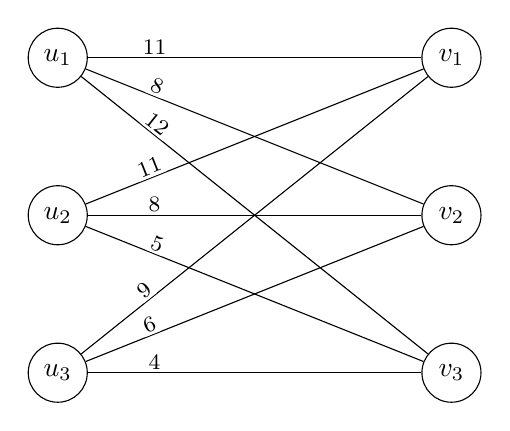
\begin{tikzpicture}[
			vertex/.style={circle, draw, minimum size=0.75cm, inner sep=0pt},
			elabel/.style={draw=none, fill=white, inner sep=1pt, font=\footnotesize},
		]
		\node[vertex] (u1) at (0, 4)   {$u_1$};
		\node[vertex] (u2) at (0, 2)   {$u_2$};
		\node[vertex] (u3) at (0, 0)   {$u_3$};
		\node[vertex] (v1) at (5, 4)   {$v_1$};
		\node[vertex] (v2) at (5, 2)   {$v_2$};
		\node[vertex] (v3) at (5, 0)   {$v_3$};

		\draw (u1) -- node[elabel, pos=0.2, above, sloped] {11} (v1);
		\draw (u1) -- node[elabel, pos=0.2, above, sloped] {8} (v2);
		\draw (u1) -- node[elabel, pos=0.2, above, sloped] {12} (v3);
		\draw (u2) -- node[elabel, pos=0.2, above, sloped] {11} (v1);
		\draw (u2) -- node[elabel, pos=0.2, above, sloped] {8} (v2);
		\draw (u2) -- node[elabel, pos=0.2, above, sloped] {5} (v3);
		\draw (u3) -- node[elabel, pos=0.2, above, sloped] {9} (v1);
		\draw (u3) -- node[elabel, pos=0.2, above, sloped] {6} (v2);
		\draw (u3) -- node[elabel, pos=0.2, above, sloped] {4} (v3);

		% Optimal matching edges
		% \draw[ultra thick, NavyBlue] (u1) -- node[elabel, pos=0.5, above, sloped] {1} (v2);
		% \draw[ultra thick, NavyBlue] (u2) -- node[elabel, pos=0.5, above, sloped] {2} (v1);
		% \draw[ultra thick, NavyBlue] (u3) -- node[elabel, pos=0.5, above, sloped] {2} (v3);
	\end{tikzpicture}
\end{center}

Start with choosing some of the edges:

\begin{center}
	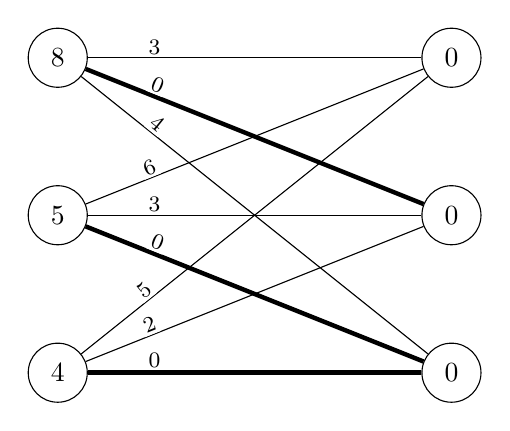
\begin{tikzpicture}[
			vertex/.style={circle, draw, minimum size=0.75cm, inner sep=0pt},
			elabel/.style={draw=none, fill=white, inner sep=1pt, font=\footnotesize},
		]
		\node[vertex] (u1) at (0, 4)   {8};
		\node[vertex] (u2) at (0, 2)   {5};
		\node[vertex] (u3) at (0, 0)   {4};
		\node[vertex] (v1) at (5, 4)   {0};
		\node[vertex] (v2) at (5, 2)   {0};
		\node[vertex] (v3) at (5, 0)   {0};

		\draw (u1) -- node[elabel, pos=0.2, above, sloped] {3} (v1);
		\draw[ultra thick] (u1) -- node[elabel, pos=0.2, above, sloped] {0} (v2);
		\draw (u1) -- node[elabel, pos=0.2, above, sloped] {4} (v3);
		\draw (u2) -- node[elabel, pos=0.2, above, sloped] {6} (v1);
		\draw (u2) -- node[elabel, pos=0.2, above, sloped] {3} (v2);
		\draw[ultra thick] (u2) -- node[elabel, pos=0.2, above, sloped] {0} (v3);
		\draw (u3) -- node[elabel, pos=0.2, above, sloped] {5} (v1);
		\draw (u3) -- node[elabel, pos=0.2, above, sloped] {2} (v2);
		\draw[ultra thick] (u3) -- node[elabel, pos=0.2, above, sloped] {0} (v3);

		% Optimal matching edges
		% \draw[ultra thick, NavyBlue] (u1) -- node[elabel, pos=0.5, above, sloped] {1} (v2);
		% \draw[ultra thick, NavyBlue] (u2) -- node[elabel, pos=0.5, above, sloped] {2} (v1);
		% \draw[ultra thick, NavyBlue] (u3) -- node[elabel, pos=0.5, above, sloped] {2} (v3);
	\end{tikzpicture}
\end{center}

Note that $v_1$ has no zero edge, we can pick $v_1$ and subtract 3 from all edges incident to $v_1$:

\begin{center}
	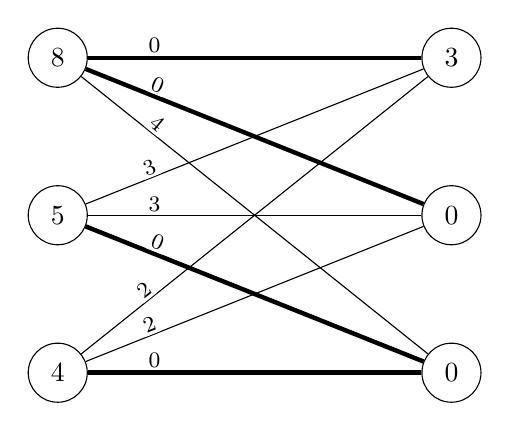
\begin{tikzpicture}[
			vertex/.style={circle, draw, minimum size=0.75cm, inner sep=0pt},
			elabel/.style={draw=none, fill=white, inner sep=1pt, font=\footnotesize},
		]
		\node[vertex] (u1) at (0, 4)   {8};
		\node[vertex] (u2) at (0, 2)   {5};
		\node[vertex] (u3) at (0, 0)   {4};
		\node[vertex] (v1) at (5, 4)   {3};
		\node[vertex] (v2) at (5, 2)   {0};
		\node[vertex] (v3) at (5, 0)   {0};

		\draw[ultra thick] (u1) -- node[elabel, pos=0.2, above, sloped] {0} (v1);
		\draw[ultra thick] (u1) -- node[elabel, pos=0.2, above, sloped] {0} (v2);
		\draw (u1) -- node[elabel, pos=0.2, above, sloped] {4} (v3);
		\draw (u2) -- node[elabel, pos=0.2, above, sloped] {3} (v1);
		\draw (u2) -- node[elabel, pos=0.2, above, sloped] {3} (v2);
		\draw[ultra thick] (u2) -- node[elabel, pos=0.2, above, sloped] {0} (v3);
		\draw (u3) -- node[elabel, pos=0.2, above, sloped] {2} (v1);
		\draw (u3) -- node[elabel, pos=0.2, above, sloped] {2} (v2);
		\draw[ultra thick] (u3) -- node[elabel, pos=0.2, above, sloped] {0} (v3);

		% Optimal matching edges
		% \draw[ultra thick, NavyBlue] (u1) -- node[elabel, pos=0.5, above, sloped] {1} (v2);
		% \draw[ultra thick, NavyBlue] (u2) -- node[elabel, pos=0.5, above, sloped] {2} (v1);
		% \draw[ultra thick, NavyBlue] (u3) -- node[elabel, pos=0.5, above, sloped] {2} (v3);
	\end{tikzpicture}
\end{center}
